\chapter{NAS Algorithm and Acceleration}

\todo{I have already written some staff about NAS so this might be redundant}

\begin{sloppypar}
Neural Architecture Search (NAS) has emerged as a powerful tool for automating the design of deep learning models, but it is often criticized for its computational overhead and time-consuming evaluations. In practical settings, especially on resource-constrained platforms, reducing the total search time becomes a critical objective. 
\newline
This chapter presents the methods developed to accelerate NAS with a particular focus on increasing evaluation throughput while preserving model quality. We employ a Genetic Algorithm (GA)-based strategy to intelligently explore the architecture space, enabling us to assess a large number of candidate models efficiently. The following sections detail the motivation, design, and implementation of our approach, as well as the enhancements introduced to further reduce search time and improve scalability.
\end{sloppypar}

\section{Memory Estimation}

As previously discussed, one of the most significant challenges in this work was designing neural network architectures that fit within the strict memory constraints of the Arduino deployment environment. Initially, the process involved generating an architecture, training it, and attempting deployment—only to discover that the model exceeded the hardware limitations. 

This trial-and-error approach proved inefficient and was quickly abandoned. To address this, we developed a memory estimation mechanism capable of predicting the resource consumption of a model based solely on its architectural configuration. This allowed us to pre-screen candidate models and discard those unlikely to meet the deployment constraints, thereby accelerating the NAS process and conserving computational resources.

In addition, based on these memory estimations, we were able to predict secondary metrics such as inference time and current consumption—values that previously required the model to be deployed in order to be measured. This advancement further streamlined the design and evaluation process.


To successfully deploy our neural network on the Arduino Nano 33 BLE Sense, we must adhere to the device's stringent resource constraints—specifically, a maximum of 256\,KB of RAM and 1\,MB of Flash memory. Any model exceeding these limits becomes undeployable, regardless of its theoretical accuracy or performance.

While the most precise method for measuring memory usage involves compiling and deploying the model onto the microcontroller to observe its runtime behavior, this process is extremely time-consuming. This is particularly impractical when evaluating thousands of candidate architectures during Neural Architecture Search (NAS). Consequently, there is a critical need for fast and reliable approximation methods capable of predicting RAM and Flash consumption without requiring actual deployment.


Based on prior research \cite{tensorflow_RamEstimation}, \cite{liberis2019neural} , we make reasonable assumptions to model
memory consumption:

• RAM usage is estimated by analyzing activation tensor sizes during inference, con
sidering their lifetimes and potential coexistence.

• Flash usage is initially approximated from the number of model parameters, then
corrected using a regression model to account for format overheads like quantization
metadata and FlatBuffer structure.

These assumptions allow us to perform fast memory estimations with reasonable accu
racy, enabling effective filtering and prioritization of architectures before committing to
the costly deployment step. To improve the quality of these estimates, empirical data
was collected and regression models were trained to correct for systematic biases in the
naïve estimators. The resulting tools are embedded in the module, ensuring that only
deployable models are selected for further optimization

Although the Arduino Nano 33 BLE Sense provides 1~MB of Flash memory and 256~KB of RAM, the usable memory available for deploying a neural network model is significantly less due to system-level overhead. This overhead arises from several essential components required for model execution and embedded functionality:

\begin{itemize}
    \item \textbf{Flash Memory Overhead:} In addition to the model weights and logic—stored in a \texttt{.h} file converted from a \texttt{.tflite} model and consuming the majority of board's memory, additional consumption arises from:
    \begin{itemize}
        \item \textbf{CMSIS-NN / Inference Functions:} Optimized functions responsible for executing the neural network layers (e.g., \texttt{arm\_nn\_softmax\_common}, \texttt{arm\_depthwise\_conv\_opt}, etc.) are stored in Flash memory. The more complex the model (i.e., more layers or operations), the more Flash these functions consume.
        \item \textbf{Arduino Sketch Code:} To deploy the model on the board, a sketch is used that includes constant variables, initialized pointers, additional libraries, static variables, and runtime logic. All of these contribute to Flash consumption.
    \end{itemize}
\end{itemize}

\newpage


\begin{itemize}
    \item \textbf{RAM Overhead:} Beyond the Tensor Arena—which is allocated specifically for intermediate buffers during inference—several other components consume RAM:
    \begin{itemize}
        \item \textbf{Main Stack} (\textasciitilde32~KB): Reserved for function calls, local variables, and handling interrupts. This ensures safe execution across diverse runtime scenarios.
        \item \textbf{Standard Library Buffers:}
        \begin{itemize}
            \item \texttt{impure\_data} (\textasciitilde2~KB) and \texttt{\_\_malloc\_av\_} (\textasciitilde41~KB): Internal allocations used by the newlib C library for dynamic memory and standard I/O handling.
        \end{itemize}
        \item \textbf{System Threads and OS Buffers:}
        \begin{itemize}
            \item \texttt{os\_timer\_thread\_stack}: Allocated for RTOS timer handling and related system threads.
        \end{itemize}
        \item \textbf{Peripheral and Communication Buffers:}
        \begin{itemize}
            \item Buffers used by \texttt{\_SerialUSB}, I2C interfaces (\texttt{Wire}, \texttt{Wire1}), and other hardware drivers consume variable RAM depending on their initialization.
        \end{itemize}
        \item \textbf{Static Objects and Runtime Metadata:}
        \begin{itemize}
            \item Instances like \texttt{\_ZZ5setupE8resolver} and static variables declared in the sketch occupy RAM during execution.
        \end{itemize}
        \item \textbf{Interrupt Handlers and Background Tasks:} RAM is also consumed by interrupt service routines (e.g., for BLE events, sensor data polling) and background OS tasks.
    \end{itemize}
\end{itemize}


Empirical measurements during deployment revealed that, in addition to the model's footprint, the following are typical overheads:

\begin{itemize}
    \item \textbf{Flash Usage:} \textasciitilde200--210~KB (depending on model size and included libraries).
    \item \textbf{RAM Usage:} \textasciitilde45--50~KB for the tensor arena and runtime state.
\end{itemize}





\clearpage

\subsection{Flash Memory Estimation}

Estimating the flash memory required to deploy a neural network model on a microcontroller is critical for resource-constrained edge computing. A common approach is to compute the flash requirement based on the number of model parameters, which represent the weights and biases that must be stored in read-only memory (ROM) \cite{pau2023tiny}.

This method is fast and easy to compute, but it doesn't accurately reflect the size of a fully converted \texttt{.tflite} model due to additional overhead such as:
\begin{itemize}
    \item Quantization calibration parameters
    \item Padding and alignment used in FlatBuffer format \cite{manor2022custom}
\end{itemize}



The initial estimation function used the following logic:
\[
\text{Estimated Flash (KB)} = \frac{\text{Total Parameters} \times \text{Data Type Size (Bytes)}}{1024}
\]

This approach uses the \texttt{count\_params()} method from Keras and assumes a constant multiplier depending on data type 1 byte as when we save the .tflite we have quantaize the model to int8 ( 1 byte)

While efficient, this method consistently underestimates the actual TFLite model size, which might allow bigger than the allowed to be trained while it will not fit in the deployment enviroment making it time consuming training something too big.

To verify accuracy, a dataset of real models was collected. Each model was:
\begin{enumerate}
    \item Built using Keras
    \item Converted to TFLite with full integer quantization
    \item Measured for actual file size in kilobytes
\end{enumerate}

The results showed a consistent non-linear gap between the estimated and actual sizes, motivating the use of a correction model.

We applied a simple linear regression model to learn the relationship between the estimated flash (param-based) and the actual flash (TFLite file size):

\[
\text{Corrected Flash Estimate} = a \cdot \text{Estimated Flash} + b
\]

Using a dataset of paired values, we trained the regression model and obtained the following parameters:
\[
\text{TFLite Size} \approx 1.1577 \cdot \text{Estimate} + 66.10
\]

 This model was saved using \textbf{joblib} and can be reused to instantly predict corrected flash estimates without invoking the TFLite converter.

 \begin{figure}[ht]
  \centering
  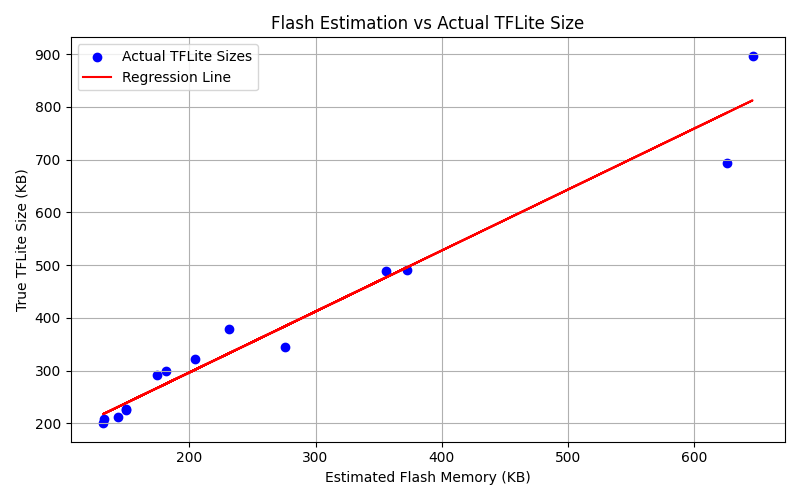
\includegraphics[width=0.85\textwidth]{Pictures/flash_regression_plot.png}
  \caption{Linear regression fit between estimated and true TFLite flash sizes.}
  \label{fig:flash-regression}
\end{figure}


Although the sample-based estimation is generally close to the actual deployment behavior, in cases where a model approaches the Flash memory limits, it is advisable to perform an early conversion to the \texttt{.tflite} format. This allows verification that the model fits within the memory constraints before proceeding with full training. The workflow consists of first converting the untrained Keras model to a TFLite version to ensure feasibility, then continuing with the regular training of the original Keras model, followed by conversion and deployment as usual.

Although this process introduces a small time overhead—typically just a few seconds—it is negligible compared to the cost of fully training a model, which can take around 20 minutes, only to later discover it cannot be deployed due to memory constraints. Conducting an early Flash feasibility check thus serves as a valuable safeguard, helping to avoid unnecessary training and conserve computational resources..

\clearpage

\subsection{Ram Memory Estimation}

During inference, each layer produces intermediate activation tensors that occupy RAM. However, not all intermediate tensors exist in memory at once – their lifetimes are limited to when they are being computed and used. A naïve approach (not reusing any buffer) would allocate a separate buffer for every intermediate tensor but this can lead to a huge memory footprint. \cite{tensorflow_RamEstimation} 


The key insight is that we can estimate the peak RAM usage by analyzing the sizes of activation tensors and understanding which ones coexist at runtime. Typically, the peak memory occurs at a layer where the largest combination of activations must be stored simultaneously. For sequential models (simple chains), this often boils down to the input and output of a single layer – once a layer’s output is produced, the previous activations can be released. \cite{liberis2019neural}

 A simplified but effective heuristic is to assume that the input and output tensors of each layer represent the concurrent memory needed during the computation of that layer, and take the maximum over all layers \cite{tensorflow_RamEstimation}. 

However, layers such as Concatenate introduce memory persistence, requiring previous activations to remain allocated until the merge operation completes. This forces multiple tensors to coexist in memory simultaneously, leading to overlapping memory demands. As a result, the real peak RAM usage can substantially exceed the simple input-output memory estimation. 

\TODO{PEAK OF each Stage , Stem Block, Refiner}

Empirical observations show that in models with frequent merging operations or consecutive high-memory layers, the actual RAM consumption can approach roughly twice the theoretical maximum estimated from single-layer analysis.

\begin{figure}[ht]
  \centering
  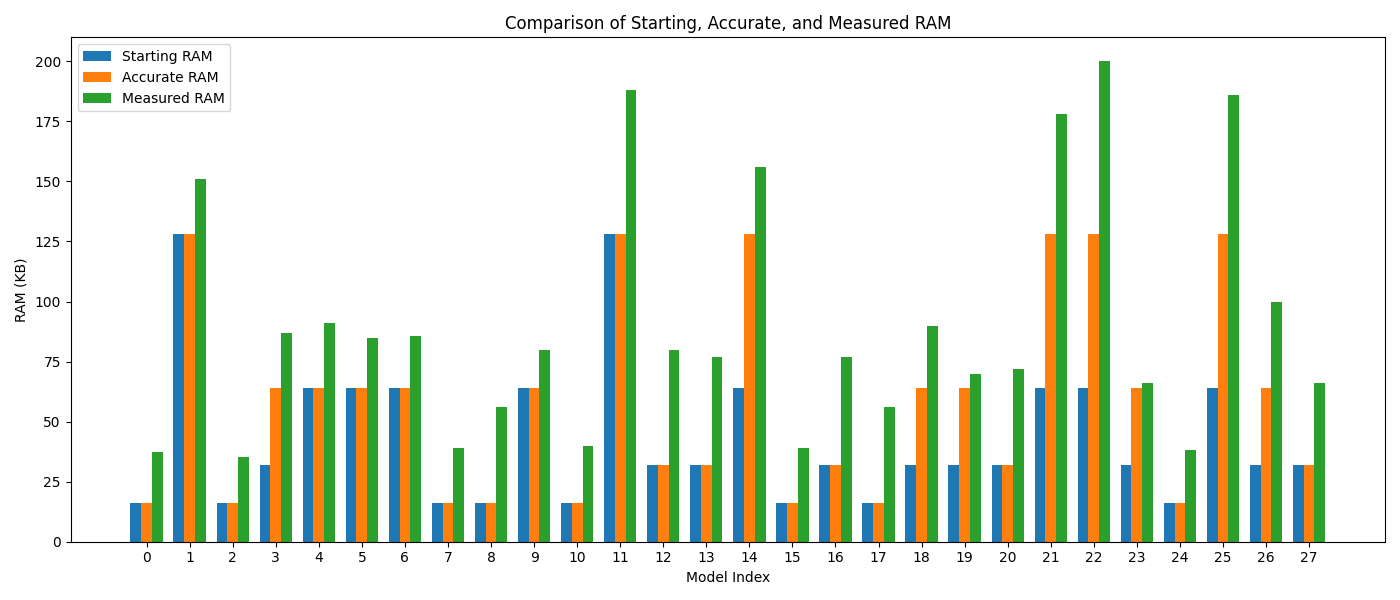
\includegraphics[width=0.85\textwidth]{Pictures/InitialAccurateMeasured.png}
  \caption{Comparison of Estimated, Accurate, and Measured RAM usage}
  \label{fig:initial-ram-comparison}
\end{figure}

While the \textit{Accurate} estimation aligns more closely with the actual measured RAM, it still tends to underestimate total memory usage due to the aforementioned memory persistence effects.

To better capture this discrepancy, we applied a similar approach as the previous chapter, creating a linear regression model between the Accurate and Measured RAM values. The resulting line—referred to as \textit{LinearRAM}—reveals a consistent pattern in the mismatch, suggesting that a correction factor can be reliably modeled.

\begin{figure}[ht]
  \centering
  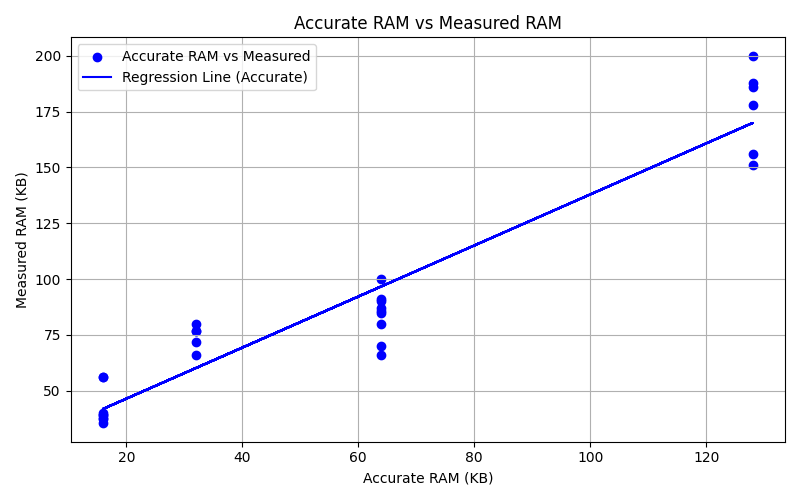
\includegraphics[width=0.85\textwidth]{Pictures/ram_accurate_vs_measured.png}
  \caption{Measured RAM vs. Accurate Estimation with Linear Regression Fit}
  \label{fig:ram-linear-regression}
\end{figure}


\clearpage


\subsection{Inference Time Estimation}
Another very interesting estimation we can do based on the already computed RAM memory is the Inference time.

Inference time refers to the time a trained model takes to produce an output from a given input – essentially the latency of a single forward-pass execution. This inference latency is strongly influenced by the model’s RAM (memory) usage, especially in embedded or microcontroller settings. Higher RAM consumption typically means the model must handle larger weight matrices or intermediate tensors in memory, leading to more data that needs to be stored and accessed during computation.
studies confirm that optimizing memory usage tends to speed up inference. For example, using fused in-place operations to reduce peak RAM footprint by about 1.6 × yielded a 1.2–2× faster inference execution in a TinyML context \cite{inferenceTime1}. Similarly, an embedded ML framework that lowered memory usage by 31\% achieved a remarkable 92\% reduction in inference latency compared to a less memory-efficient baseline~\cite{inferenceTime1}.


Those assumptions were confirmed after our test, finding a Linear coorelation between the actual Measured RAM of the model and the inference time needed to produce the result.

\begin{figure}[ht]
  \centering
  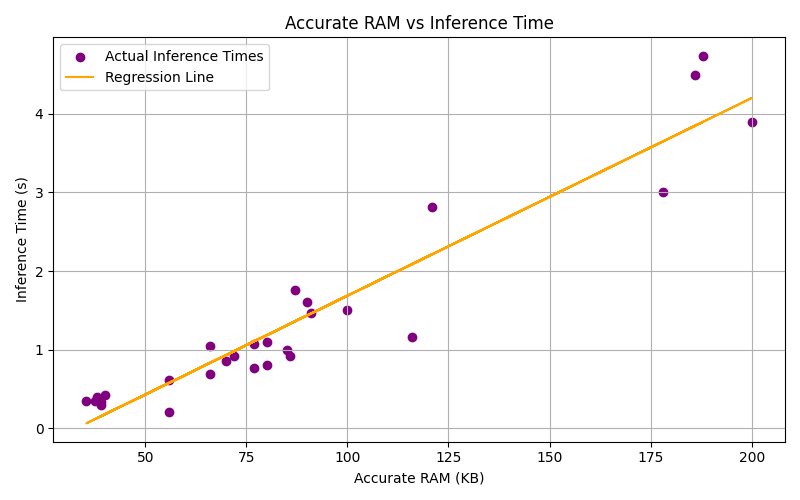
\includegraphics[width=0.85\textwidth]{Pictures/inference_time_regression_plot.png}
  \caption{Linear Corelation between RAM and inference time.}
  \label{fig:inference time}
\end{figure}

\clearpage


\subsection{Current Estimation}


\TODO{Section to be added when current is estiamted}

\section{Model Comparison}
After the creation of the models in each new generation in the GA, we face the challenge on how to correctly choose the best models as parents for the upcoming generations and how to accelerate this procedure. So in the section the Tournament Selection and RankNet will be explained on how they tackle those issues. 


\TODO{Performance STOP}

\subsection{Tournament Selection}
Tournament Selection (TS) is a genetic operator in which a small subset of individuals is chosen at random and the fittest among them is selected as a parent \cite{hussain2020trade}. 
Concretely, one chooses a tournament size \textit{k} and repeatedly samples \textit{k} individuals from the population. The individual with the highest fitness in each sampled group is declared the winner and used for reproduction \cite{hussain2020trade}.

Tournament selection inherently preserves population diversity and thus supports generalization. Because selection is based on competition within small random samples, occasionally sub-optimal individuals can win and propagate their genes \cite{hussain2020trade}.

In effect, TS avoids the extreme elitism of always picking the single best, which can lead to premature convergence. A well-designed selection should maintain diversity to avoid getting stuck in local optima \cite{filipovic2003fine}.

By keeping a variety of architectures in the gene pool, TS enables the GA to explore multiple promising regions of the search space. This broader search helps prevent overfitting to any one metric and tends to produce more robust CNN designs.


\subsection{RankNet}

In our initial approach, we attempted to train all the models and then use the TS, to create the new generation. After some experiments, we find out that this approach was extremely time-consuming to fully train a model only to drop it in the tournament selection. For this reason we introduced \textit{RankNet} to be able to predict the best model even without training.

\TODO{Look at this a bit more}

\textbf{RankNet} is a pairwise ranking model originally developed for learning-to-rank tasks (e.g. search result ranking). It uses a shared neural network to map each input (here, an architecture embedding) to a score, then models the probability that one item is better than another by a sigmoid on the score difference \cite{RankNet}.

A key enabler for RankNet in NAS is a fixed-length embedding of each architecture that captures its structure. Recent works use graph-based embeddings; for example, Graph2Vec treats a neural network’s computational DAG as a “document” of rooted subgraphs (analogous to words) and learns a vector representation such that architectures with similar subgraph patterns are mapped close together in embedding space \cite{RankNet}.

In our case, the embedding strategy is much simpler and more lightweight. We use the hyperparameters defined in the NAS search space, assuming a fixed architecture template across all candidate models. Since only the internal parameters (e.g., kernel sizes, filter counts, strides) vary, this parameter-based embedding is both valid and appropriate. All numerical values are normalized and collected into a fixed-size vector, ready to be fed into the RankNet surrogate model.

Once the architectures are embedded, a RankNet model is trained on a set of fully evaluated networks. Rather than regressing absolute accuracy values, RankNet learns to predict *relative* performance: given a pair of architecture embeddings, it estimates the probability that one outperforms the other. This pairwise comparison allows RankNet to learn a ranking function such that $f(x_i) > f(x_j)$ when model $i$ performs better than model $j$. This strategy is advantageous because modeling relative fitness is often more robust and data-efficient than predicting absolute scores.

However, during the early stages of evolution, the RankNet model is not yet reliable due to limited training data. To address this, we adopt two key strategies:

\begin{enumerate}
    \item \textbf{Progressive Refinement:} As the search progresses, we accumulate an increasing number of fully trained models. After each generation, we retrain the RankNet using the new pairwise comparisons, allowing the model to incrementally improve its ranking accuracy.
    
    \item \textbf{Active Correction:} During tournament selection, if RankNet favors an untrained model over a trained one, we train the untrained model and compare their true performance. If RankNet’s prediction was incorrect, we retain the better-performing model and use the misprediction as a penalty signal for RankNet—effectively updating its training data to reflect this mistake in the next retraining cycle.
\end{enumerate}

These mechanisms help RankNet adapt over time and increase the reliability of its predictions, ultimately leading to a more efficient and informed neural architecture search.






\section{Speed-Up in Training}

Once a model is selected—either as part of the initial population or through evolutionary selection—it must undergo full training to evaluate its true performance. Given the potentially large number of candidate architectures evaluated during the search, reducing training time becomes crucial for overall efficiency. Therefore, we implemented several optimization strategies to accelerate the training process, without significantly compromising the quality of the resulting models. These strategies aim to minimize unnecessary computational overhead, enabling faster feedback loops within the NAS cycle and more rapid convergence.

\subsection{Early Stopping}

Research indicates that during CNN training, the initial few epochs often yield the most significant gains in model learning, strongly shaping the network’s eventual accuracy. In other words, a large portion of a CNN’s final validation performance is determined early in training. The following are key findings from credible sources that support this idea.

In an analysis of “critical learning periods,” the authors found that “the first few epochs are critical for the creation of strong connections” in a neural network, after which these connections “do not appear to change during additional training.” They conclude that this initial learning phase “plays a key role in determining the outcome of the training process.” In practice, most of the network’s representational capacity and generalization ability is established in these early epochs \cite{achille2017critical}

In Figure ~\ref{fig:val_accuracy}, it can be depicted the normalized validation accuracy of couple of TakuNet models through the epochs. 
It is clear that the accuracy above 65\% of the total validation is achieved within the first epochs of training.
In order to speed up the entire NAS algorithm, a Custom Callback method was introduced, which measured the validation accuracy of the model at the important the 20\% of the total epochs. If the validation accuracy did not exceed a specific threshold, the algorithm abandons the model as it is pointless to spend more training time to a non-optimal model based on its constraints.

\begin{figure}[ht]
    \centering
    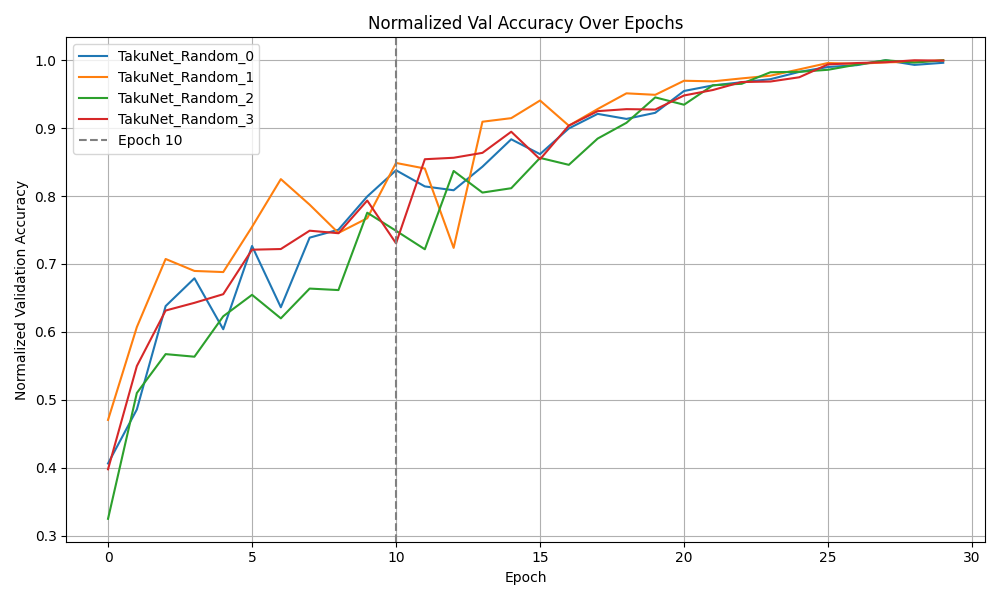
\includegraphics[width=0.85\linewidth]{Pictures/val_accuracy_comparison.png}
    \caption{Normalized validation accuracy curves for TakuNet variants. Around epoch 10, the models typically achieve more than 65\% of their total validation performance.}
    \label{fig:val_accuracy}
\end{figure}

\clearpage

\subsection{Learning Rate Scheduling}
To accelerate convergence and improve generalization, we employed a cosine annealing learning rate schedule with a linear warmup phase of 5 epochs. This strategy adjusts the learning rate dynamically across training: starting from a small value, rising linearly during warmup, and then decaying smoothly according to a cosine function relative to the total number of epochs. 

The cosine function used ,inspired by \cite{loshchilov2016sgdr} : 

\begin{equation}
\text{lr}(t) = \eta_0 \cdot \frac{1}{2} \left( 1 + \cos\left( \frac{\pi (t - T_\text{warmup})}{T_\text{total} - T_\text{warmup}} \right) \right),
\end{equation}

where:
\begin{itemize}
  \item \( \eta_0 \) is the initial learning rate,
  \item \( T_\text{warmup} \) is the number of warmup epochs,
  \item \( T_\text{total} \) is the total number of training epochs,
  \item \( t \) is the current epoch number.
\end{itemize}


Cosine learning rate schedules have been widely adopted in modern image classification models such as ResNet, DenseNet, and MobileNet, and are considered state-of-the-art for datasets like CIFAR-10 and CIFAR-100~\cite{lewkowycz2021decay}. Studies show that cosine decay leads to faster convergence and slightly improved final accuracy compared to traditional step-based schedules.

As illustrated in Figure~\ref{fig:val_accuracy_diff_epochs}, for the TakuNet model, increasing the number of training epochs beyond 10 does not significantly improve validation accuracy, given the Learning Rate Scheduling technique used. This saturation effect aligns with the theoretical behavior of cosine decay: once the learning rate approaches zero, further updates become minimal. Given that each epoch takes approximately one minute to complete, it is computationally efficient to limit training to around 10 epochs—achieving nearly optimal results in a fraction of the training time and is sufficient to be able to compare models.



\begin{figure}[ht]
    \centering
    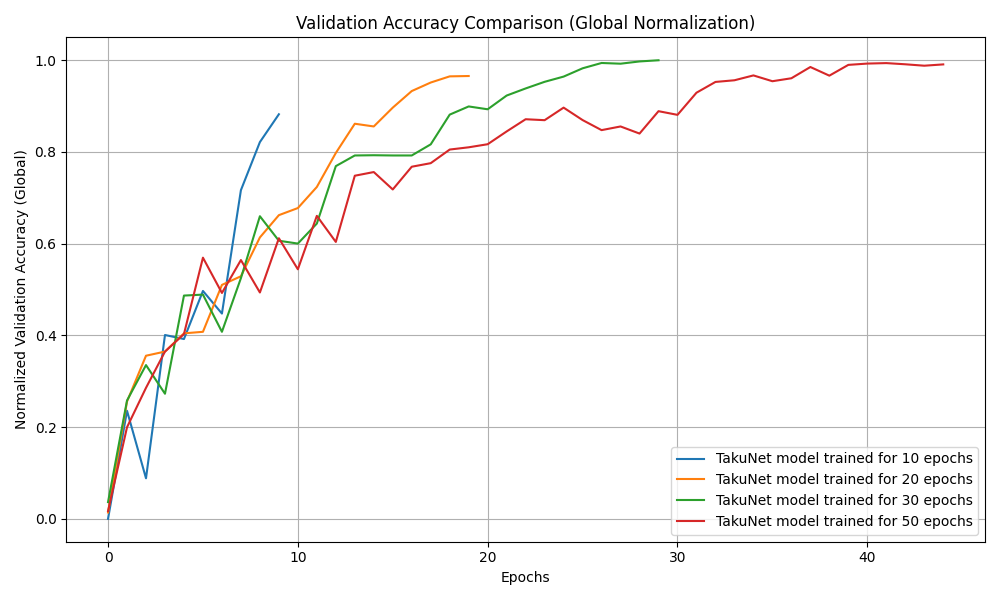
\includegraphics[width=0.85\linewidth]{Pictures/val_accuracy_comparison_global.png}
    \caption{Normalized Validation accuracy(based on highest recorder accuracy) of TakuNet trained for different number of epochs }
    \label{fig:val_accuracy_diff_epochs}
\end{figure}